\documentclass[a4j,dvipdfmx]{jsarticle}

\usepackage[dvipdfmx]{graphicx}
\usepackage{amsmath,amssymb}
\usepackage{siunitx}
\usepackage{ascmac}
\usepackage[subrefformat=parens]{subcaption}
\usepackage{fancyhdr}
\usepackage{otf}
\usepackage[dvipdfmx]{hyperref}
\usepackage{pxjahyper}

\pagestyle{headings}

% \renewcommand{\thesubsection}{\arabic{subsection}}
\renewcommand{\headrulewidth}{1pt}
\renewcommand{\Re}{\operatorname{Re}}
\renewcommand{\Im}{\operatorname{Im}}

\newcounter{basic_quastion}\setcounter{basic_quastion}{1}
\newcommand{\basicquestion}{{\large 基本問題\hspace{1mm}\huge\fbox{\textbf{\arabic{basic_quastion}}}\addtocounter{basic_quastion}{1}}\thispagestyle{fancy}\lhead{$\Sigma$基本問題}\rhead{\thepage}\cfoot{}\quad}


\title{Quuノート ー微分積分\ajRoman{1}ー}
\date{最終更新 2023/12/01}
\author{責任者 Quu}

\begin{document}
    \maketitle
    \thispagestyle{empty}
    \centerline{\textbf{概要}}
    \noindent
    微分積分学入門についてのノート。\\
    主に、一変数の極限、一変数の微分・積分、実数の無限級数について扱う。
    
    \clearpage
    \tableofcontents
    \clearpage
    
    \part{前提知識}
    \vspace{\stretch{1}}
    \begin{screen}
        微分積分を学ぶうえで前提となる知識をまとめた。微分積分は主に関数の微分・積分について扱うわけだから、ある程度の関数の扱い方も知っておく必要がある。
        そのほか数の種類についてや閉区間・開区間、極限についてもまとめてある。極限は微分積分を学ぶ際にいたるところに出てきて、陰から支える縁の下の力持ち的な役割を持つ。極限は一見すると
        代入と同じように見えるが、実は違う。極限は代入だと都合が悪い時にありがたみが実感できる。極限に関連して、無限という概念も登場する。
    \end{screen}
    \clearpage
    \section{様々な`数'と数直線}
        \subsection{数の種類}
            数学を勉強するうえで、様々な数が登場する。まず一番初めに思いつくのが$1,2,3...$といった\textbf{自然数}である。
            次の自然数に$0$と負の符号をつけたものを加えた\textbf{整数}が考えられる。整数同士で足し算、引き算、掛け算を行っても
            その値は整数である。このことを\textbf{和、差、積について閉じている}という。これは$a,b\in \mathbb{Z}$となる任意の$a,b$
            について
            \begin{equation}
                a+b , a-b , a\times b \in \mathbb{Z}
            \end{equation}
            が成り立つことを意味している。

            一方割り算は整数の中に閉じていない。\footnote{例えば$1\div 2$など。}しかし、$0.5,3.14$などの\textbf{有理数}まで数を拡張すれば、その中に商は閉じている。
            つまり、$a,b \in \mathbb{Q}$となる任意の$a,b$について
            \begin{equation}
                \frac{a}{b} \in \mathbb{Q}
            \end{equation}
            となる。よって、数を有理数まで拡張すれば\textbf{四則について閉じている}ことがわかる。

            さらに数の拡張を考えよう。たとえば$x^2-2=0$を満たす$x$について考えてみるには、数を\textbf{無理数}まで拡張しなければならない。
            一般の二次方程式の解も
            \begin{equation}
                x = \frac{-b\pm \sqrt{b^2-4ac}}{2a}
            \end{equation}
            と有理数だけでは表現できないことがわかる。無理数には$\pi,e\footnote{自然対数の底またはネイピア数と呼ばれる。具体的な値は$e=2.71...$}$などの\textbf{超越数}もふくむ。

            私たちの生活の中では有理数と無理数をあわせた\textbf{実数}があれば十分事足りるが、数学の世界ではそうもいかない。先ほどの二次方程式についてより深く調べてみると、
            解を持たない条件(根号の中身が負)があることがすぐに分かる。例えば、$x^2+1 = 0$は$x^2 = -1$と変形できるが、二乗して負になるような数は実数のうちには存在しない。
            よってこの方程式は\textbf{解なし}となる。がしかし、ここで
            \begin{equation}
                i = \sqrt{-1}
            \end{equation}
            となる`数'を定義してあげると、方程式は$x=\pm i$となり、$(実数)+i$を含めた範囲に解をもつことがわかる。
            この数は、今までの実数とは異なる数であり、実数との和,差は直接計算できない。一般に実数$a,b$と$i$を用いて
            \begin{equation}
                z = a + bi
            \end{equation}
            として表した$z$を\textbf{複素数}といい、$i$を虚数単位という。さらに$a$を$z$の実部、$b$を$z$の虚部といい、それぞれ
            $a=\Re z,b=\Im z$と表す。

            先ほど、二次方程式の解を有理数だけでは表現できないといったが、実は無理数を含めてもできない。この複素数を含めることで初めてすべて表現できるようになるのだ。\footnote{もちろんこれで数の拡張が終わるわけではない。しかし微分積分を学ぶうち間は複素数まで拡張すれば事足りる。}
        \subsection{数直線}
            では、数の大小関係をわかりやすくするためにはどうすればよいだろうか。視覚的にわかりやすくするためには数直線を用いればよい。
            \begin{figure}[h]
                \centering
                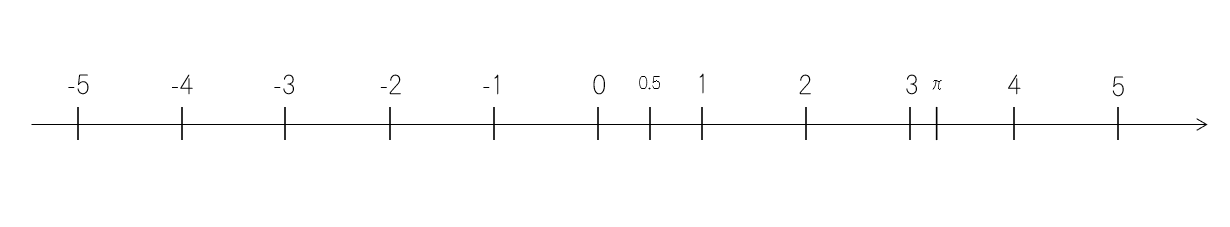
\includegraphics[keepaspectratio,scale=0.5]{img/QuuNote/NumLine_1.png}
                \caption{数直線}
            \end{figure}
            
            上の例では、整数、有理数、無理数の一部を記載している。当然書いてある数以外も数直線の中には含まれている。
            むしろ、数の点の集まりとして数直線を捉える方がイメージがわきやすいかもしれない。
            ここで注意しなければならないのは、この数直線上に複素数$(\Im z\neq 0)$は含まれないといけないということである。
            数直線は\underline{実数を表す}直線なので、実数より(集合的に)大きい複素数のすべては含むことができないのである。

            では実数も含めた複素数はどう表せばよいのか。答えは単純で実数の軸\footnote{これを実軸と呼ぶ。}とは別の軸\footnote{虚軸という。}を
            加えればよい。つまり複素数は平`面'上で表せられるのである。\footnote{この平面を複素平面という。いつものy-xグラフとは見た目は同じだが感覚が違うので注意。}  
            \newpage
        \subsection{開区間・閉区間}
            実数が数直線上の一点で表せることはすでに前項で述べた。では点に続いて次は区間について考えていこう。

            区間は大きく二つある。それらはそれぞれ\textbf{開区間}、\textbf{閉区間}と呼ばれる。これらの違いは端点を含むかどうかで、
            逆に言えば端以外は同じである。例えば、$1<x<2,1\leq x\leq2$について前者は端点$x=1,2$を含まず、後者は端点を含むのである。
            端点を含まない場合が開区間、端点を含む場合が閉区間である。

            閉区間、開区間を数直線上で表すにはどうすればよいだろうか。これも数直線と同様に区間の端から端まで線を引けばよい。注意しないといけないのが
            端点で、区間が開区間か閉区間かによって端点を書き分けないといけない。開区間のときは$\circ$、閉区間のときは$\bullet$と書けばよい。

            \begin{figure}[h]
                \centering
                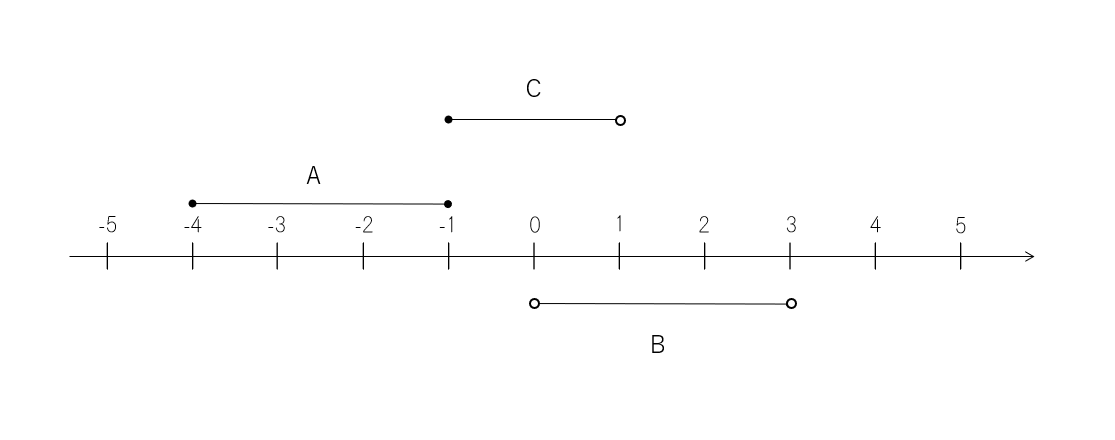
\includegraphics[keepaspectratio,scale=0.7]{img/QuuNote/IntervalLine.png}
                \caption{開区間と閉区間}
            \end{figure}
            例えば上図の例をみてみると、$A,B,C$の三つの区間がある。それぞれ$-4\leq x\leq -1,0<x<3,-1\leq x<1$となる。
            今までは不等号を用いて区間を表現してきたが\footnote{厳密に言えば区間は集合なので、不等号を用いて区間を表現するという言い方は適切ではない。}、もっと簡潔に$(\hspace{1mm}),[\hspace{1mm}]$を用いて表現する方法もある。
            この表現方法を使えば、$A,B,C$はそれぞれ$[-4,-1],(0,3),[-1,1]$と表せる。$(\hspace{1mm})$が等号を含まない、$[\hspace{1mm}]$が
            等号を含む、というわけである。

            では、値が無限に続く(例えば実数全体など)場合はどう表現すればよいのか。この場合は無限大の記号$\infty$を用いて$(-\infty,\infty)$などと表せばよい。\footnote{この方法を使えば、a以上の実数などの場合でも$[a,\infty)$と表せばよいことがわかる。}
            \clearpage
            
        \noindent
        \basicquestion 以下問に答えよ。

        \paragraph{問1}以下の主張のうち正しいものには〇を、間違っているものには×をつけよ。
            \begin{enumerate}
                \item $\sqrt{9}$は無理数である。
                \item 有理数は全て分数の形で表せる。
                \item $i$は複素数である。
                \item 有理数の集合は$\mathbb{Q}$として表し、無理数の集合は$\mathbb{N}$で表す。
                \item 自然数全体の集合(区間)は$(0,\infty]$である。
            \end{enumerate}
        \paragraph{問2}以下の区間について、数直線上に示せ。もし数直線上に記されていない数字が出てくる場合はそれも記載せよ。
            \begin{figure}[h]
                \centering
                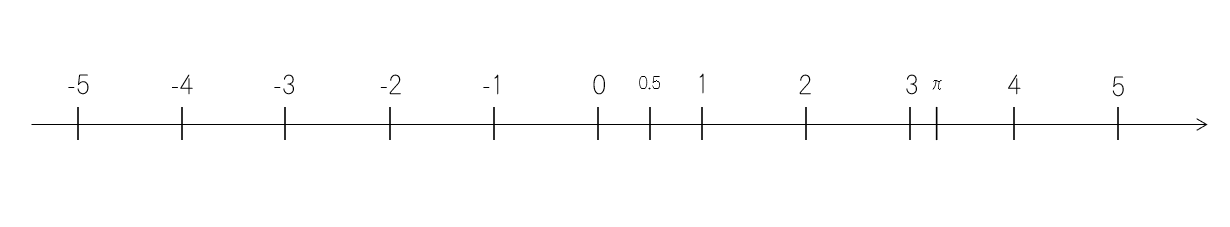
\includegraphics[keepaspectratio,scale=0.6]{img/QuuNote/NumLine_1.png}
                \caption{数直線}
            \end{figure}

            $1.\quad [2,3]$\hspace{3mm}
            $2.\quad (3,5)$\hspace{3mm}
            $3.\quad [-5,\pi]$\hspace{3mm}
            $4.\quad (-2,0.5]$\hspace{3mm}
            $5.\quad [-1,0)$\hspace{3mm}
            $6.\quad (-\infty,0)$\hspace{3mm}
            $7.\quad [0,\infty)$\hspace{3mm}
        \clearpage
        
        \section{関数の性質}
            \subsection{偶関数・奇関数}
                一般の関数$f(x)$について、$f(-x)=f(x)$を満たすものを\textbf{偶関数}、$f(-x)=-f(x)$を満たすものを\textbf{奇関数}という。
                もちろん全ての関数が偶関数・奇関数のどちらかであるというわけではない。しかし、全ての関数は偶関数と奇関数の和で表せられること
                が知られている。\\

                関数が偶関数・奇関数である場合のグラフはどうなるだろうか。まずは偶関数から考えてみると、定義より$x>0$と$x<0$の点において$f$は
                同じ値を取るわけであるから、グラフはy軸に対して対象になるはずである。つぎに奇関数について考えてみよう。これも定義より$x>0$と$x<0$の
                点において、$f$はx軸に対してそれぞれ対象に点を取るはずである。つまり、グラフは原点に対して点対象になるはずである。\\

                偶関数の例となる関数は、$x^2,\cos x,a(\text{定数関数})$などがあげられる。奇関数の例となる関数は、$x,\sin x,\tan x$などがあげられる。
                各自でグラフソフトなどでグラフを見てみるとよい。
            \clearpage
            \subsection{べき関数}
                関数のなかでもっともなじみやすいのが、$f(x)=x^n$であろう。例えば$x$は一次関数、$x^2$は二次関数と呼ばれる。
                別に$n$は自然数に限らなくてもよい。$x^{\frac{1}{2}}=\sqrt{x}$は指数が自然数ではないが、これもべき関数の一つである。
                $n$が自然数のうちは、関数の定義域について特別意識をする必要はない。しかし$n=\frac{1}{2}$などのように指数が有理数であったり、
                $n=-1$のように指数が負の値を取る場合には定義域に十分注意する必要がある。このように、一般に$f(x)=x^n$で表される関数を\textbf{べき関数}という。

                次に関数のグラフについて、グラフ描画ソフトを用いて数式を入力すると以下のようになる。
                \begin{figure}[h]
                    \centering
                    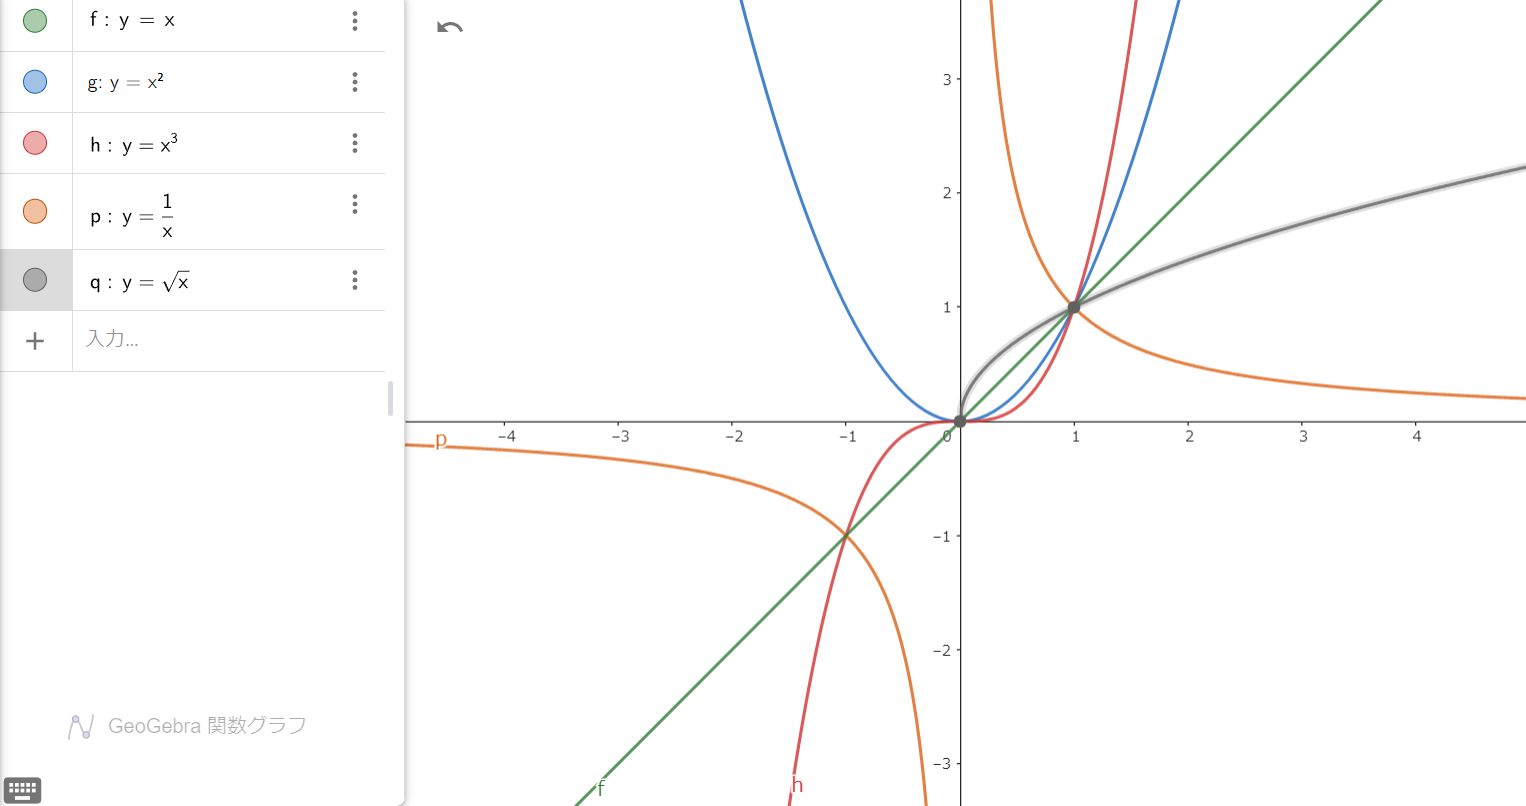
\includegraphics[keepaspectratio,scale=0.5]{img/QuuNote/PowerFuncGraph.png}
                    \caption{べき関数グラフ}
                \end{figure}

                図からも$\sqrt{x}$が$x<0$で定義されないことがわかる。また、$x^2$と$\sqrt{x}$は$y=x$を軸にして線対象になっており、
                $x^2$と$\sqrt{x}$は互いに\textbf{逆関数}であることがわかる。


    \clearpage
    \part{微分}

    \clearpage
    \part{積分}

    \clearpage
    \part{無限級数}

\end{document}